\chapter{Cadre général du stage et parcours préparatoire}
    
\rhead{Cadre général du stage et parcours préparatoire}
\lfoot{\leftmark}

\section{Introduction}
Ce chapitre présente le cadre général du stage de fin d'études. Nous commençons par une présentation de l'organisme d'accueil, le groupe SQLI, avant de détailler le parcours d'intégration et les activités préliminaires réalisées en amont du projet.

%--------------------------SQLI------------------------------
\section{Présentation de l'organisme d'accueil}
\subsection{Groupe SQLI}
Fondé en 1990, SQLI est un groupe européen de services digitaux spécialisé dans la conception d’expériences digitales innovantes. Il accompagne de grandes marques internationales dans leur transformation numérique, en les aidant à créer de la valeur à travers le digital.

Le groupe SQLI compte près de 3 400 collaborateurs répartis dans plusieurs pays, notamment en France (Paris, Lyon, Toulouse, Bordeaux, Rouen, Nantes, Lille), en Suisse(Lausanne, Genève), au Luxembourg, en Belgique (Bruxelles), aux Pays-Bas, au Maroc(Rabat, Casablanca, Oujda), ainsi qu’en Espagne (Barcelone) et à Dubaï.

Le groupe accorde une importance particulière aux méthodologies agiles, et conduit la majorité de ses projets selon le cadre SCRUM. Cette organisation agile contribue à sa performance, avec un chiffre d’affaires ayant atteint 251,2 millions d’euros en 2023, en constante progression depuis plusieurs années. \cite{logo:sqli1}

SQLI compte plus de 2000 clients, grands comptes et PME, issus de divers secteurs d’activité, tels que :
\begin{itemize}
    \item Les services
    \item Les banques et assurances
    \item Les administrations et services publics
    \item La distribution
    \item L’immobilier
    \item Les transports
    \item Les télécommunications
\end{itemize}

La figure 1.1 présente la répartition de SQLI dans le monde.

\begin{figure}[H]
    \centering
    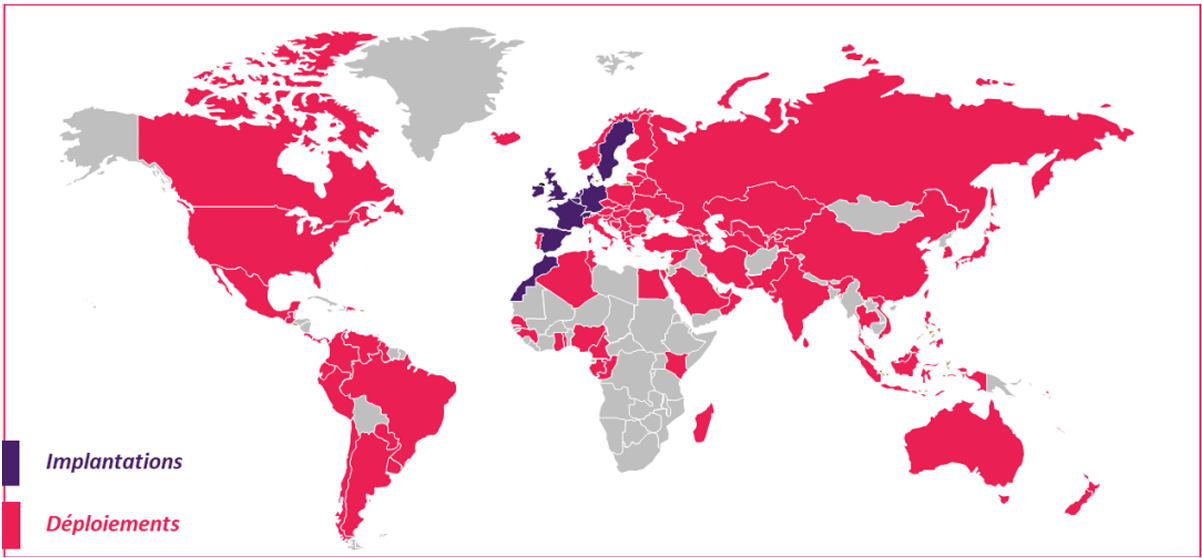
\includegraphics[width=1\textwidth]{images/sqlirepartition.png}
    \caption{Présence de SQLI dans le monde}
\end{figure}

\subsection{Fondamentaux SQLI}
L'agence SQLI Rabat dispose d'un département Data \& IA, qui regroupe des expertises en data engineering, data science et en analyse avancée des données pour répondre aux besoins métiers. L'agence mobilise une grande diversité de technologies pour accompagner ses clients, tout en partageant les mêmes fondamentaux organisationnels et humains que l'ensemble du groupe SQLI.

SQLI place au cœur de sa culture d'entreprise des valeurs fortes telles que le respect, l'esprit d'équipe, l'authenticité, l'engagement et le goût du challenge. Les collaborateurs sont encouragés à innover, à proposer des idées et à s'impliquer activement dans les projets.

Trois axes majeurs structurent la démarche du groupe :
\begin{itemize}
    \item L’excellence opérationnelle, appuyée par la méthodologie CMMI, avec une certification de niveau 3 obtenue dès 2006.
    \item La relation client, fondée sur l’écoute et la compréhension des enjeux métiers, à travers le programme qualité interne Business CMM.
    \item L’innovation, portée par le laboratoire interne 6mmx, qui conçoit des solutions performantes et génératrices de valeur, déployées à l’échelle du groupe.
\end{itemize}

\subsection{Organigramme de Sqli}
Lasociété SQLI dispose d’un organigramme illustrant sa structure globale et l’organisation de ses différents services.

Autrefois indépendants, les centres de Rabat et Oujda ont récemment été fusionnés dans le cadre d’une nouvelle réorganisation interne, donnant naissance à une entité unique : ISC Maroc (Industrialized Services Center).

Cette restructuration vise à renforcer la synergie entre les équipes et à offrir une vision plus cohérente et centralisée de l’organisation.

La figure \ref{fig:organi} présente l’organigramme adopté par SQLI
\begin{figure}[H]
    \centering
    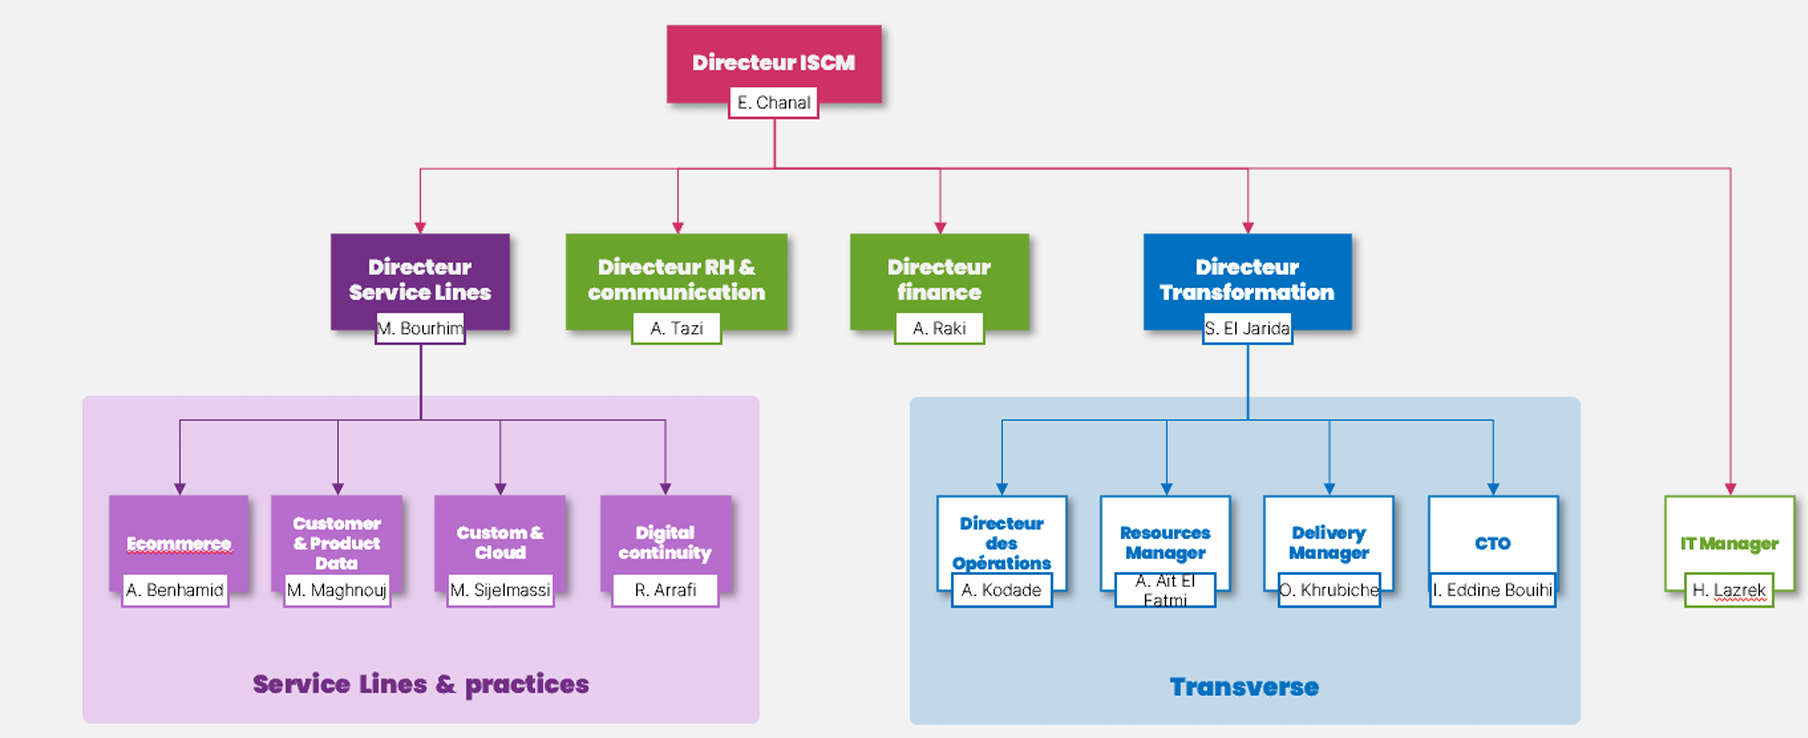
\includegraphics[width=1\textwidth]{images/organigramme.png}
    \caption{Organigramme de SQLI}
    \label{fig:organi}
\end{figure}

\subsection{Mission et domaines d’expertise}
SQLI a pour mission de créer des expériences digitales à forte valeur ajoutée pour les grandes marques, en les accompagnant dans leur transformation numérique. Le groupe se distingue par son approche centrée sur l’innovation et l’expérience utilisateur, en proposant des solutions adaptées aux besoins spécifiques de chaque client.

SQLI intervient dans plusieurs domaines clés :
\begin{itemize}
    \item \textbf{E-commerceetExpériences Digitales: } Création de plateformes e-commerce, sites web interactifs, et applications mobiles. 
    \item \textbf{Data et Intelligence Artificielle: } Exploitation des données pour améliorer la performance des entreprises grâce à l’analyse de données, l’automatisation, et le machine learning.
    \item \textbf{Stratégie Digitale: }  Conseil et accompagnement dans la définition et la mise en œuvre de stratégies digitales pour améliorer la compétitivité.
    \item \textbf{Transformation Digitale: }  Intégration de nouvelles technologies et optimisation des processus pour une meilleure efficacité opérationnelle.
\end{itemize}

\subsection{Partenaires de SQLI}
SQLI s’appuie sur un réseau de partenaires technologiques stratégiques afin d’enrichir son offre de services et de garantir à ses clients des solutions performantes, innovantes et adaptées aux standards du marché.
La figure \ref{fig:part} représente les logos de quelques
partenaires technologiques de SQLI. \cite{logo:sqli2}
\begin{figure}[H]
    \centering
    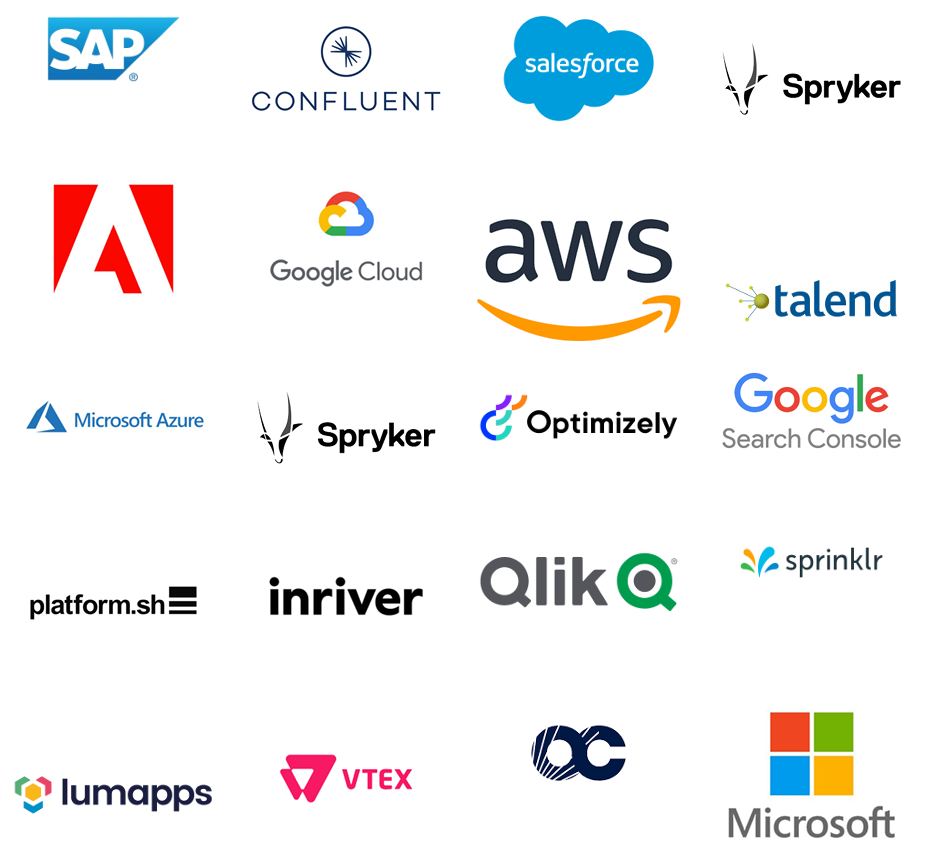
\includegraphics[width=1\textwidth]{images/partenaires.png}
    \caption{Logos des principaux partenaires de SQLI}
    \label{fig:part}
\end{figure}
%------------------------------Activités--------------------------
\section{Intégration et activités préliminaires}
Chaque année, SQLI organise le concours national e-Challenge, un événement destiné à renforcer les liens entre l’entreprise et les établissements d’enseignement supérieur. Cette initiative a pour but d’offrir aux futurs lauréats une immersion concrète dans le monde
professionnel, à travers la réalisation de projets de fin d’études (PFE) avec une réelle perspective d’embauche.

Dans ce cadre, le processus de sélection débute par un concours technique sur la plateforme HackerRank, consistant en une épreuve de 3 heures axée sur des problématiques
d’algorithmique, de développement et de logique. Les candidats retenus passent ensuite un entretien technique et RH, d’une durée d’environ une heure, afin d’évaluer à la
fois leurs compétences techniques et leur adéquation avec les valeurs de l’entreprise.
\subsection{Formation sur les technologies Big Data et Cloud }
À l'issue du processus de sélection, les candidats admis bénéficient d'un programme de formation intensif d'une durée de quatre semaines, dispensé via la plateforme Udemy. Cette formation vise à consolider les compétences techniques nécessaires au bon déroulement du stage, en couvrant les technologies clés de l'écosystème Data \& IA de l'entreprise.

Le programme s'articule autour de quatre modules complémentaires. 
\begin{itemize}
    \item Le premier module consiste en un bootcamp complet en SQL et Snowflake, axé sur les fondamentaux de l'analyse de données, notamment la manipulation de requêtes complexes et l'exploitation des fonctionnalités avancées de Snowflake.
    \item Le deuxième module est consacré à l'analyse de données avec Pandas et Python, permettant de maîtriser le traitement, le nettoyage et la transformation de jeux de données volumineux.
    \item Le troisième module porte sur Azure Databricks et Spark SQL avec Python, offrant une introduction à l'environnement cloud Azure ainsi qu'au traitement distribué des données à grande échelle.
    \item Le quatrième module constitue une formation avancée sur Snowflake, couvrant l'ensemble de ses fonctionnalités, de l'architecture interne à l'optimisation des performances.
\end{itemize}
Ce parcours de formation a permis d'acquérir une maîtrise solide des outils et technologies mobilisés tout au long du projet de fin d'études, tout en facilitant l'intégration au sein de l'équipe Data \& IA de l'agence.

\subsection{Préparation à la certification Snowflake}
En parallèle du programme de formation, une phase de préparation à la certification SnowPro Core (C03) a été engagée. Cette certification, délivrée officiellement par Snowflake, atteste d'un niveau de compétence solide sur les concepts fondamentaux de la plateforme, couvrant notamment l'architecture, le chargement et la transformation des données, la gestion des entrepôts virtuels, la sécurité ainsi que l'optimisation des performances.

La préparation s'est appuyée sur plusieurs ressources complémentaires. Les connaissances acquises lors des modules de formation Udemy, en particulier les deux modules dédiés à Snowflake, ont constitué une base essentielle. Cette base a été renforcée par l'étude approfondie de la documentation officielle de Snowflake, ainsi que par la réalisation de nombreux examens blancs permettant de se familiariser avec le format des questions et d'identifier les axes d'amélioration.

Cette démarche a abouti à l'obtention de la certification SnowPro Core (C03), validant ainsi une maîtrise des fonctionnalités clés de la plateforme Snowflake. Cette certification représente un atout significatif dans le cadre du projet de fin d'études, dans la mesure où Snowflake constitue l'un des piliers technologiques de la solution mise en œuvre.

La figure \ref{fig:certisnow} présente une copie du certificat obtenu.
\begin{figure}[H]
    \centering
    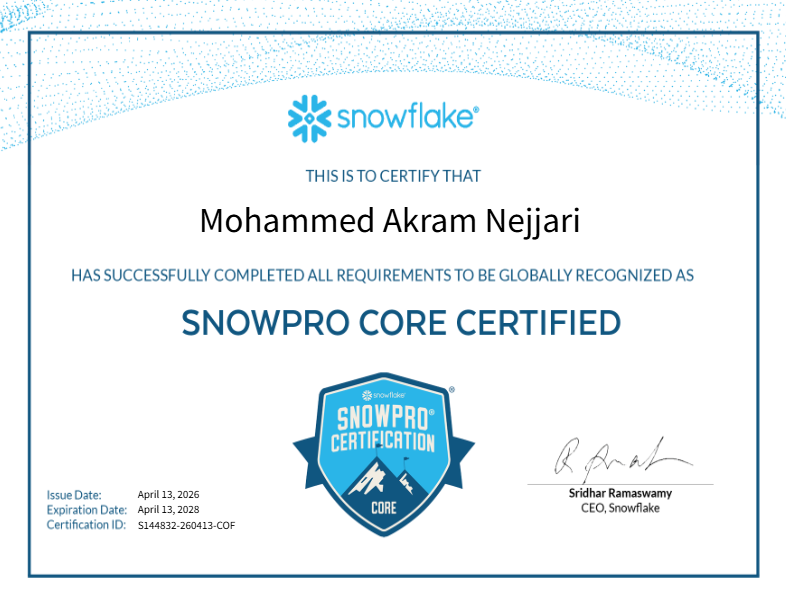
\includegraphics[width=1\textwidth]{images/certifsnow.png}
    \caption{Certificat SnowPro Core (C03)}
    \label{fig:certisnow}
\end{figure}

\subsection{Participation au Hackathon}
Dans le cadre des activités préliminaires au stage, une participation à un hackathon interne organisé par SQLI a été réalisée. Cet événement portait sur l'utilisation de Snowflake Cortex et s'inscrivait dans le contexte d'un cas d'usage réel pour un client majeur de l'entreprise.

Le hackathon était structuré en deux volets complémentaires. Le premier volet, orienté Data Engineering, consistait à mettre en place les pipelines de préparation et de transformation des données nécessaires à l'alimentation de la solution. Le second volet, dédié à l'intelligence artificielle, portait sur l'exploitation des modèles de langage avancés (LLM) intégrés à Snowflake Cortex afin d'automatiser des tâches complexes, notamment l'analyse et la prédiction.

L'objectif était de concevoir une solution complète de traitement et d'analyse intelligente des incidents, en s'appuyant sur une approche de Root Cause Analysis (RCA) appliquée aux tickets JIRA. Cette solution visait à identifier automatiquement les causes profondes des incidents récurrents, réduisant ainsi le temps de diagnostic et améliorant la prise de décision.

Cette expérience a constitué une mise en pratique concrète des compétences acquises lors de la formation, tout en offrant une première confrontation avec les exigences d'un projet réel en environnement professionnel.

La figure \ref{fig:certihackath} présente une copie du certificat de participation à ce hackathon.
\begin{figure}[H]
    \centering
    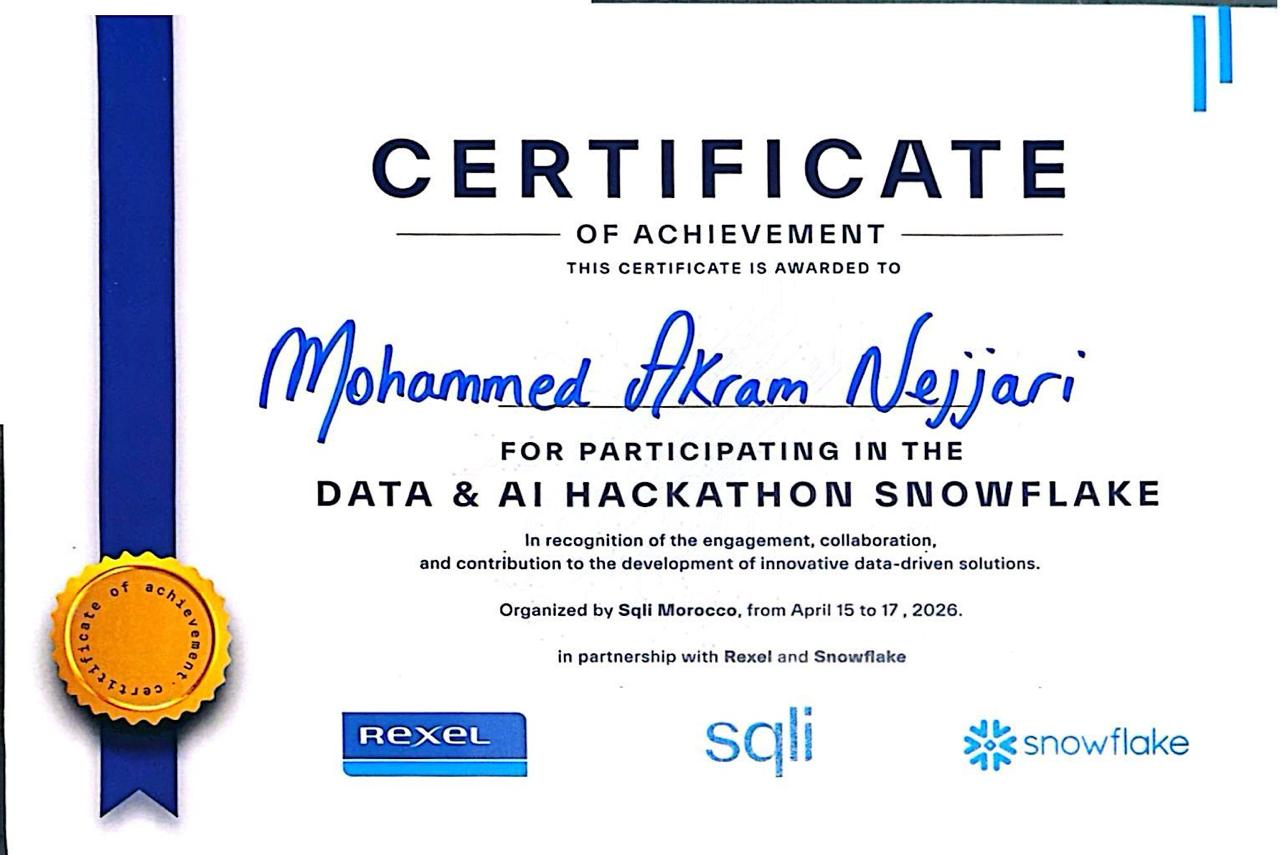
\includegraphics[width=1\textwidth]{images/hackathon.jpeg}
    \caption{Certificat de participation au hackathon}
    \label{fig:certihackath}
\end{figure}

\subsection{Compétences acquises}
L'ensemble des activités préliminaires menées au cours de cette phase d'intégration a permis de développer un socle de compétences à la fois techniques et transversales, directement mobilisables dans le cadre du projet de fin d'études.

Sur le plan technique, les compétences acquises couvrent plusieurs domaines clés. La maîtrise de la plateforme Snowflake, validée par l'obtention de la certification SnowPro Core (C03), constitue un acquis majeur, englobant l'architecture cloud, la gestion des entrepôts virtuels, le chargement et la transformation des données ainsi que l'optimisation des performances. La formation a également permis de consolider les compétences en SQL avancé pour l'interrogation et l'analyse de données complexes, en Python appliqué à la manipulation de données à travers la bibliothèque Pandas, ainsi qu'en traitement distribué via Apache Spark SQL sur l'environnement Azure Databricks. Par ailleurs, la participation au hackathon a offert une première expérience pratique avec les modèles de langage intégrés à Snowflake Cortex.

Sur le plan transversal, cette phase a favorisé le développement de compétences en travail collaboratif et en gestion du temps, notamment lors du hackathon où la coordination au sein de l'équipe et le respect des délais étaient essentiels. La capacité à appréhender rapidement de nouvelles technologies et à les appliquer dans un contexte concret a également été renforcée, de même que l'aptitude à analyser une problématique métier et à proposer une solution adaptée.

Ces compétences constituent un socle solide pour aborder le projet de fin d'études dans les meilleures conditions.

\section{Conclusion}
Ce chapitre a permis de présenter l'organisme d'accueil ainsi que le parcours préparatoire au stage, incluant la formation, la certification SnowPro Core (C03) et la participation au hackathon. Ces étapes ont constitué une base solide pour aborder le projet de fin d'études, dont le contexte général sera détaillé dans le chapitre suivant.